\title{%
  \Huge{\textbf{Interactive Tool for Teaching Hindley-Milner Type Inference through Visualisation}}
  \\
  \Large{Final report\\~\\~\textbf{Adam Jones}\\~Department of Computer Science\\~University of Warwick}
}

\documentclass[a4paper,fleqn,12pt]{article}

\usepackage[]{geometry}
\usepackage[utf8]{inputenc}
\usepackage[UKenglish]{babel}
\usepackage[UKenglish]{isodate}
\usepackage{amsmath}
\usepackage{amsfonts}
\usepackage{amssymb}
\usepackage{amsthm}
\usepackage{graphicx}
\usepackage{chngpage}
\usepackage{calc}
\PassOptionsToPackage{hyphens}{url}
\usepackage{hyperref}
\usepackage[nameinlink]{cleveref}
\usepackage{fancyhdr}
\usepackage{titletoc}
\usepackage[explicit]{titlesec}
\usepackage{natbib}
\usepackage[dvipsnames]{xcolor}
\usepackage[sc]{mathpazo}
\linespread{1.05} 
\usepackage[T1]{fontenc}
\usepackage{minted}
\usepackage{ragged2e}
\usepackage{adjustbox}

\hypersetup{
	colorlinks=true,
	linkcolor=black,
	urlcolor=black,
	citecolor=black
}

\definecolor{lightgrey}{rgb}{0.95,0.95,0.95}
\setminted{bgcolor=lightgrey}
\setmintedinline{bgcolor=lightgrey,escapeinside=||,mathescape=true}

\let\parencite\citep

\setlength{\parindent}{0mm}
\setlength{\parskip}{\medskipamount}
\renewcommand\baselinestretch{1.2}

\cleanlookdateon

\pagestyle{plain}
\renewcommand{\headrulewidth}{0.0pt}

\makeatletter
\fancypagestyle{plain}{
	\fancyhf{}
	\fancyhead[RE,RO]{\thepage}
	\fancyhead[LE,LO]{\textit{Interactive Tool for Teaching HM Type Inference through Visualisation}}
}
\makeatother

\begin{document}

\makeatletter
\begin{titlepage}

\LARGE \@title \\
\Large \\[1.5cm]

\vfill 

\begin{adjustwidth}{-\oddsidemargin-1in}{-\rightmargin}
  \centering
  
\includegraphics[width=\paperwidth]{line.png}
\end{adjustwidth}

\vspace*{-3.5cm}

\end{titlepage}
\makeatother

\pagestyle{plain}




TODO: Abstract
\section{Introduction}\label{id:h.6k9gcmunzldy}
Types are common features of many programming languages. Generally, types are bounds on program constructs (such as variables, expressions and functions) that limit what valid values they may take and how they should be interpreted within the program, however different languages use types differently. Most type systems include primitive data types such as integers, booleans and characters as well as composite types such functions from one type to another and lists of a type.

Type checking is the process by which a language’s compiler or interpreter validates that a program obeys the rules of the language’s type system. When a violation is detected, such as providing a boolean to a function accepting an integer, a type error is raised.

Type checking is primarily used to catch bugs in program code, preventing unexpected behaviour. A simple example of this is function application: functions’ types specify how they can be called which ensure some pre-conditions are met, such as the arguments being of an expected type. This allows function implementers to safely assume the data is of that type, and prevents function users calling the function with invalid arguments.

Type checking can happen either at compile time (static type checking) or runtime (dynamic type checking).

Compile-time type checking prevents many type errors from occurring at runtime. This is particularly useful when code paths may not be well tested or frequently used, as runtime checks only surface type errors when the problematic code is executed. Additionally, knowing types at compile-time allows for better tooling that improves developer productivity. For example, IDEs may use type information to suggest and perform automated refactorings \citep{ref1}, automatically generate documentation \citep{ref2} and autocomplete statements \citep{ref3}.

Compile-time type checking requires the program code to have enough information to validate its type safety. This may be in the form of type annotations or typed variable and function declarations. However, specifying types manually can be time-consuming and potentially difficult as it is additional work for the programmer, and large composite types can be especially difficult to determine and tedious to repeatedly write.

A type inference algorithm for a programming language’s type system can determine types automatically, which improves productivity by allowing programmers to get the best of types without having to explicitly specify them. Because of this, type inference is used in many popular programming languages with expressive type systems including Haskell, Rust and TypeScript.

An understanding of type inference would help computer scientists write cleaner code and debug type errors. However, few universities have core modules on type systems (although they may be touched on in programming curriculums) and there are limited easy-to-understand teaching resources on type inference. Therefore, many computer science graduates will be missing a useful understanding of how type inference actually works.

The goal of this project is develop a system to visualise the type inference process, with the aim of improving undergraduate students’ knowledge about it.

To achieve this, we develop a teaching resource that explains how type inference algorithms work for functional languages. An interactive web application allows students to enter expressions and view the results of a type inference algorithm, along with the steps taken to get to that result. This is particularly useful in the context of modules teaching functional languages such as Haskell which perform similar type inference.
\subsection{Related work}\label{id:h.2mwaav7jkal4}
There have been previous attempts to build visualisation and teaching tools related to type systems.

{\centering \begin{figure}[h!]
  \centering
  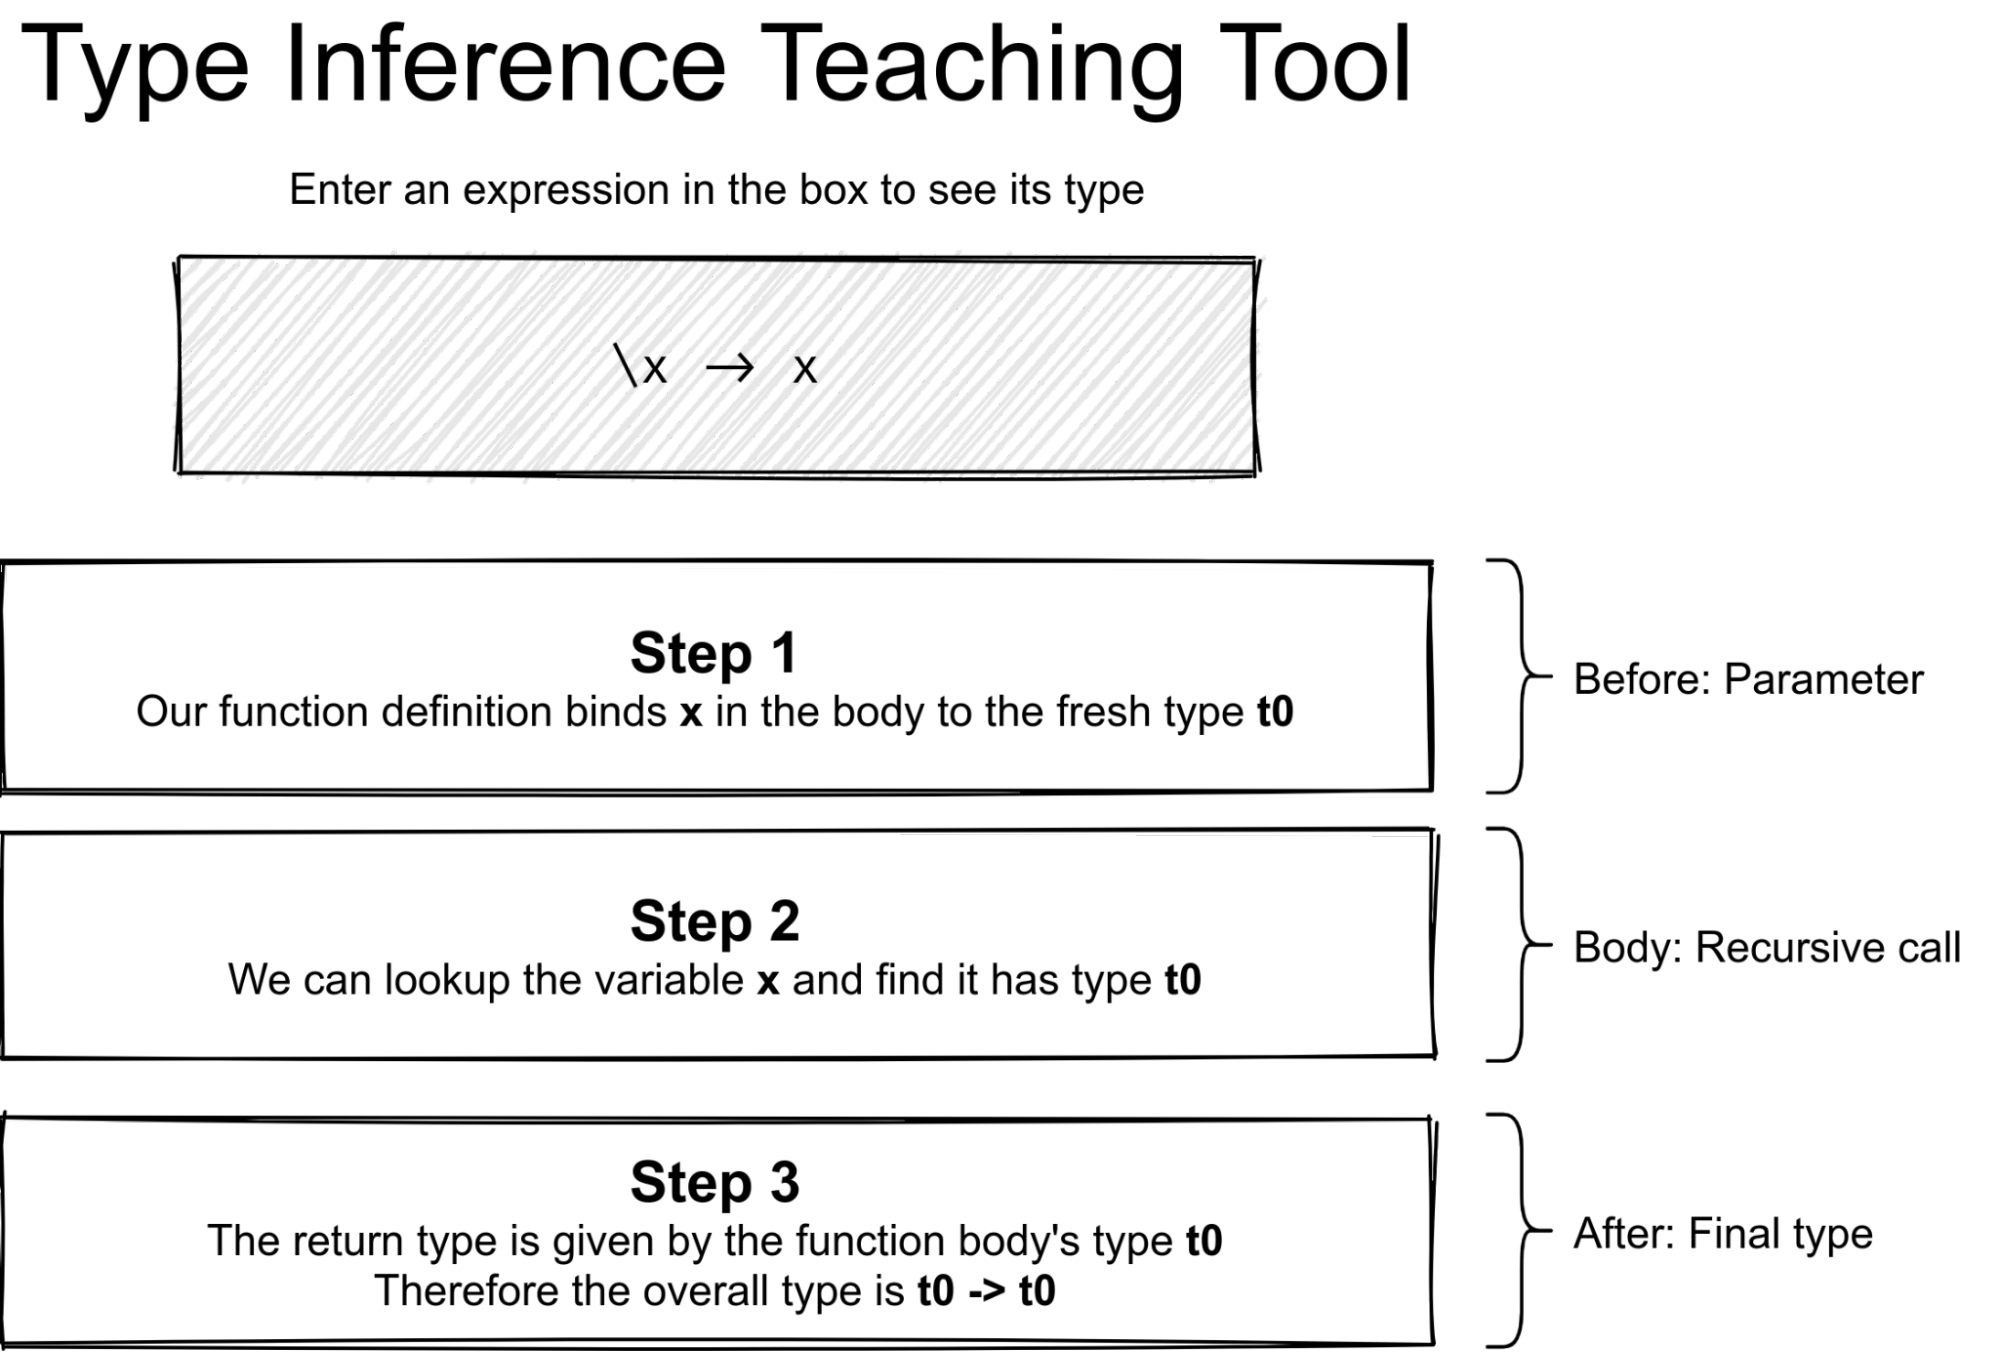
\includegraphics[width=0.770\linewidth]{images/image9.png}
  \caption{Screenshot of results from TypeTool, taken from their paper}
\end{figure} \par}

One example is TypeTool by~\cite{ref4}, which visualises type inference through a web application. Users enter an expression in a custom expression language, submit a request to a server and are redirected to a page displaying an initial syntax tree, a final syntax tree and an overall substitution. By allowing users to enter their own expressions, students can explore how the systems work in different cases to gain an intuitive understanding of the concepts.

TypeTool’s authors found in teaching the University of Porto’s functional programming course that the tool was “especially useful for students, because it helps to understand the type systems of the most common typed functional languages” and that “[presenting] the basis of type inference technology [...] significantly improved the way students deal with type errors because they understand the type system.”

However, TypeTool’s parsing and type inference is done server-side so there is a delay between the user entering an expression and seeing the result. While short, a delay reduces the ease-of-use and may discourage users from trying many different expressions. Both delayed feedback and the lack of step-by-step explanations reduce learning quality \citep{ref5}, particularly in the area of rule learning.~\cite{ref6} showed that immediate explanatory feedback is most effective at learning how to apply rules in computer programming. It also lacks step-by-step explanations, and it is unclear whether it supports processing incorrectly-typed expressions.

In addition, the tool is now inaccessible as the server hosting the application is no longer running and the source code has not been published.

Another tool in the area of visualising type systems was developed by~\cite{ref7}. It is a visual functional programming system which shows types during function application for a subset of Standard ML, used to teach first year undergraduate students. However, this did not explicitly show the type inference process and as a desktop application rather than web app it is less accessible to lecturers and students. It also didn’t support key functional language constructs such as function declarations and let bindings, and required significant explanation before using the tool to understand its output.

{\centering \begin{figure}[h!]
  \centering
  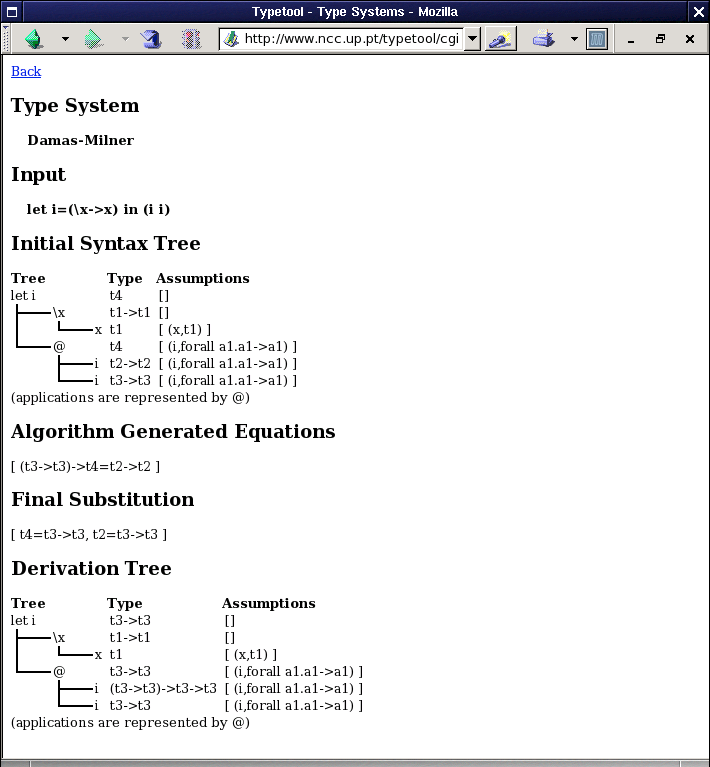
\includegraphics[width=0.797\linewidth]{images/image2.png}
  \caption{Screenshot of Yung and Michaelson's tool, taken from their paper}
\end{figure} \par}

NiMo \citep{ref8} is a graphical programming language related to functional data processing which allows users to reason about the flow of data through a program. The types of data and processes can be inspected in NiMoToons, and type inference is performed over the network of components. However, larger expressions can become complicated and be difficult to interpret. While NiMo performs type inference internally it is not a key focus to the end-user, and as such does not explain its steps. Additionally, it is harder to relate back to more commonly used, textual functional languages like Haskell.

{\centering \begin{figure}[h!]
  \centering
  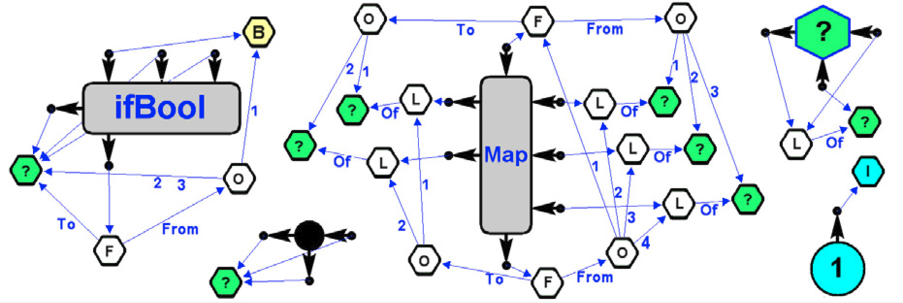
\includegraphics[width=0.960\linewidth]{images/image7.png}
  \caption{A diagram showing the types of some variables in NiMo, taken from their paper}
\end{figure} \par}

\cite{ref9} implemented a successful teaching tool, named TILC, for visualising lambda-calculus parse trees in order to help with teaching lambda-calculus to undergraduate students. They noted that to develop an intuitive understanding, students would benefit from  experimenting with lambda-calculus and that “a tool that deals with all these aspects in a friendly and graphical manner incentivises [experimentation]”. TILC was successful, with the module organisers of ‘programming paradigms’ at the Universitat de Girona having a “good experience of using this tool in the course lectures and as a downloadable tool for students”. The authors suggested extending TILC to show types and type inference would have pedagogical value.

To summarise, types aid the construction of correct programs and type checking can detect issues in programs, either at compile-time or runtime. Type inference is a method often used alongside compile-time type checking to determine types in a program, an understanding of which could benefit computer scientists in writing and debugging programs. Some solutions exist which give students a better idea about types, however they either have significant limitations or do not explicitly cover type inference. In this report, we present an interactive web application for teaching type inference.
\section{Background}\label{id:h.ebjyqi73zdyo}
\subsection{$\lambda$-calculus}\label{id:h.odw4vku9eizz}
A $\lambda$-calculus is a representation of computation. The first $\lambda$-calculus set out by~\cite{ref10}, often viewed as the canonical $\lambda$-calculus, simply has variables, function abstraction and application.

For this project, we will consider a calculus with five constructs to build expressions from. As a formal grammar:

\begin{figure}[h!]
  \centering
  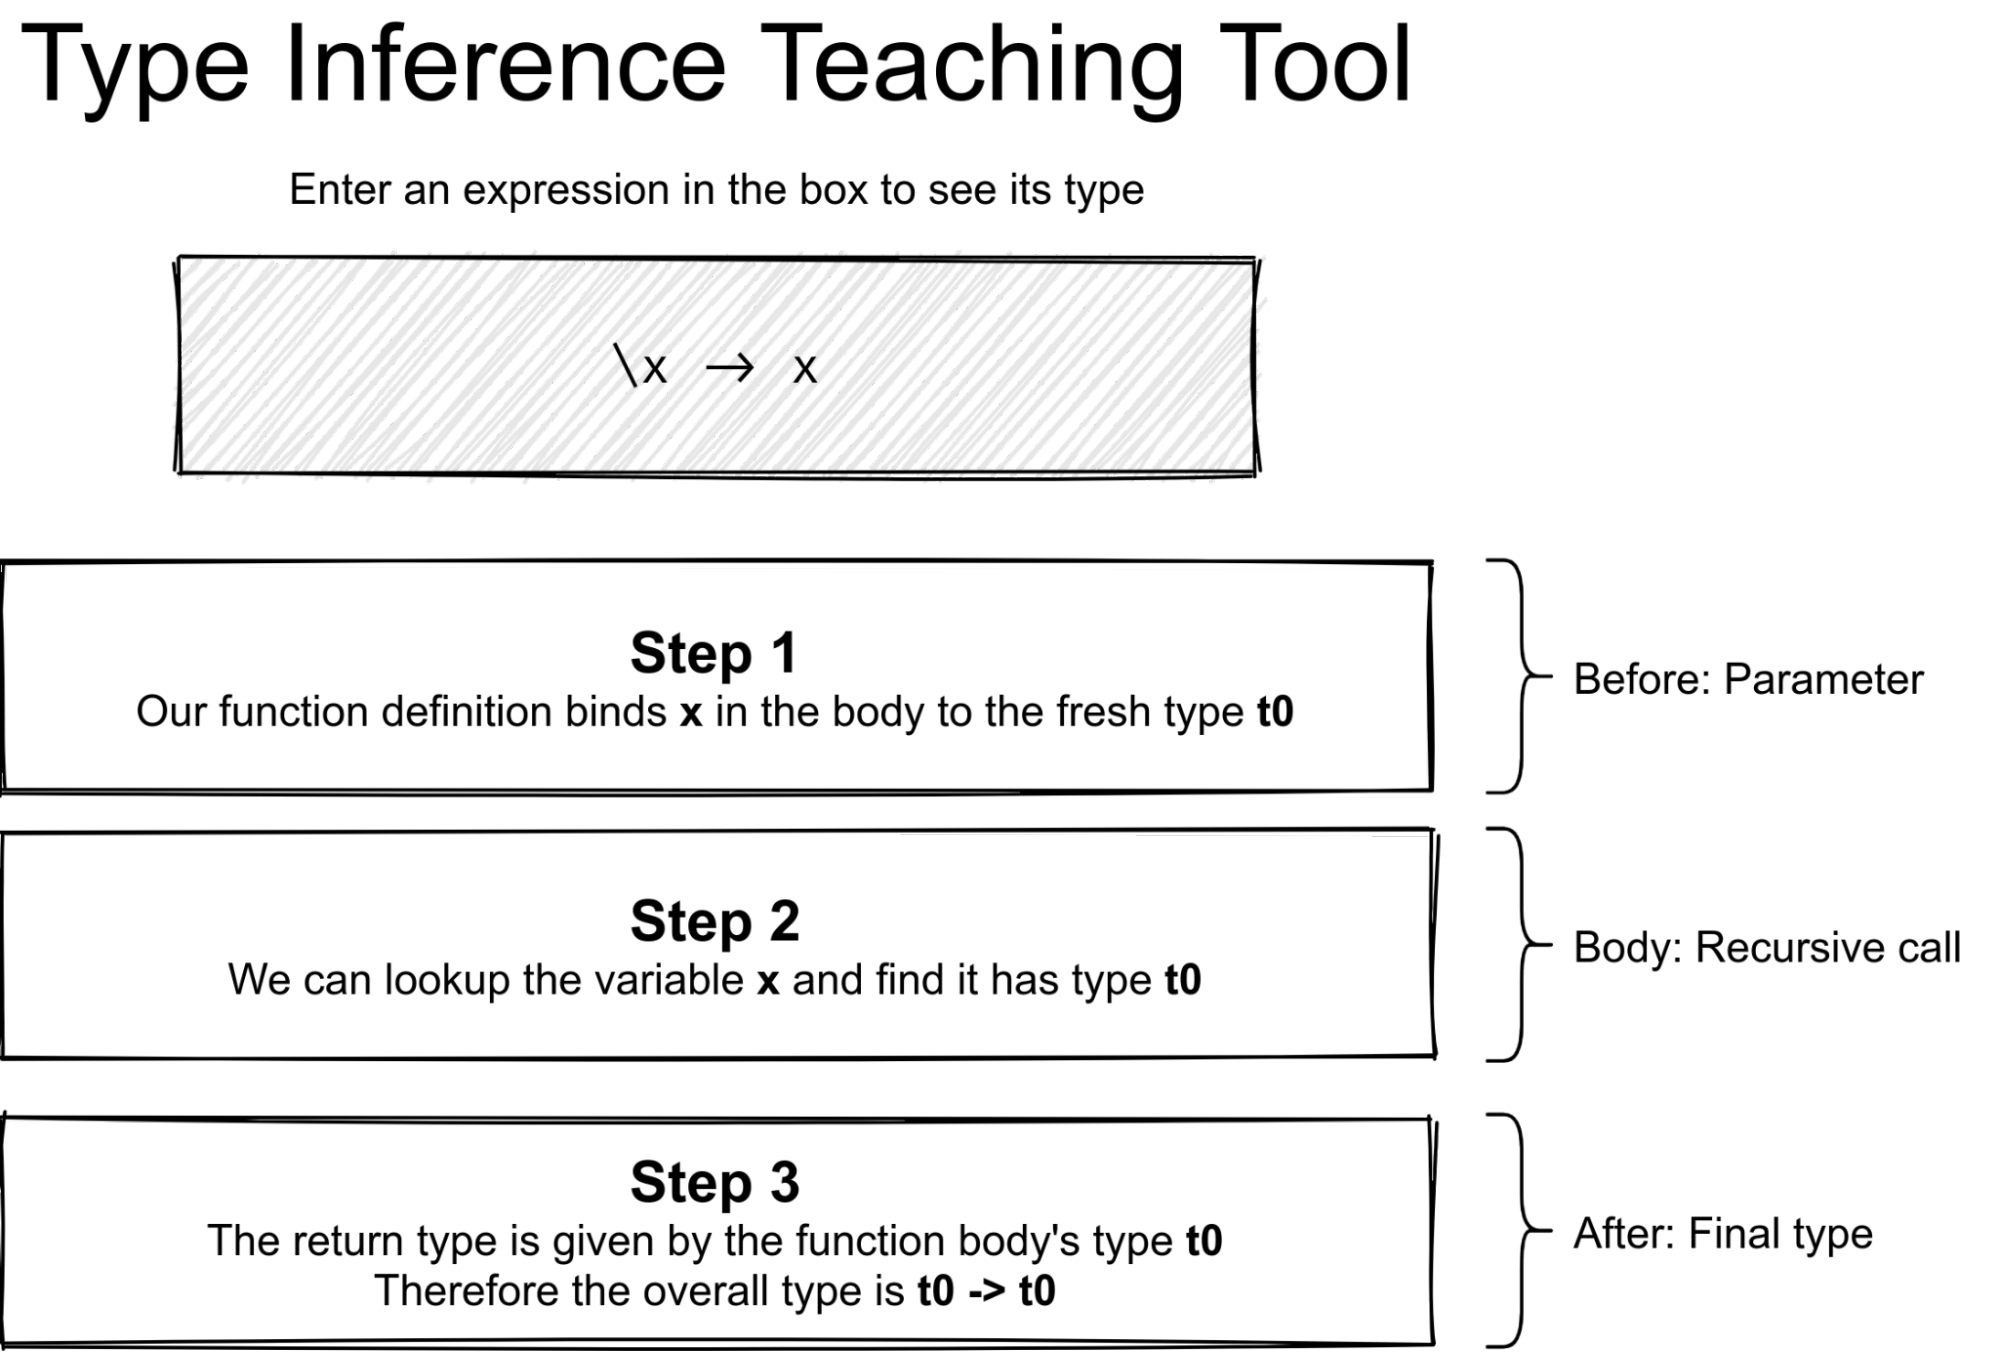
\includegraphics[width=0.510\linewidth]{images/image8.png}
\end{figure}
    | c constant

TODO: latex-ify the above, move constant to top

For example, consider the expression \mintinline{text}{|($\lambda$x. x) y|}

It has variables \mintinline{text}{|x|} and \mintinline{text}{|y|}. Variables may be bound or free (unbound). Here \mintinline{text}{|x|} is bound as it is a parameter in the function abstraction, and \mintinline{text}{|y|} is free as there is nothing which binds it. This can be thought of in a similar way to how variables in most imperative programming languages have a scope where they are defined or undefined.

The function abstraction mentioned is the \mintinline{text}{|$\lambda$x. x|} part. This defines an anonymous function which given an argument (before the full stop) \mintinline{text}{|x|} simply returns (after the full stop) \mintinline{text}{|x|}, i.e. the identity function. A function to add three to an input might be written \mintinline{text}{|$\lambda$x. x + 3|} (although many of the most fundamental $\lambda$-calculi do not have such explicit notions of addition or numbers).

Functions may be returned by other functions, which enables functions to have the appearance of taking multiple arguments. For example \mintinline{text}{|$\lambda$x. ($\lambda$y. x)|} can be viewed as a function which takes two arguments and returns the first one, even though really it is a function taking one argument which returns a function taking another argument for a result. Here explicit brackets have been given for clarity, but they aren’t necessary. Additionally, sometimes multiple arguments like this are written together, so \mintinline{text}{|$\lambda$x. ($\lambda$y. x)|}, \mintinline{text}{|$\lambda$x. $\lambda$y. x|} and \mintinline{text}{|$\lambda$xy. x|} all mean the same thing.

Finally, the function application is actually applying the function \mintinline{text}{|$\lambda$x. x|} to the argument \mintinline{text}{|y|}. In $\lambda$-calculus evaluation is performed via $\beta$-reductions. In our example this could be done by substituting the argument \mintinline{text}{|y|} for parameter \mintinline{text}{|x|} in the body of the function \mintinline{text}{|x|}, resulting in \mintinline{text}{|y|}:

This expression’s construction can be represented as an abstract syntax tree:

TODO: tree diagram of the expression

In addition to these three constructs, the \mintinline{text}{|let|} construct allows binding a value to a variable in an expression. For example \mintinline{text}{|let x = 3 in x + x|} binds \mintinline{text}{|x|} to the value \mintinline{text}{|3|} in \mintinline{text}{|x + x|}.

A \mintinline{text}{|con|} construct is added to represent literal constants, such as numbers or booleans like \mintinline{text}{|3|} and \mintinline{text}{|True|}.

$\lambda$-calculi have been extensively studied, often using formal inductive definitions. For example, the inductive definition for the set of free variables (\mintinline{text}{|var|}s not bound by function abstraction or let statements) is:
\begin{itemize}
  \item \mintinline{text}{|con|}: $FV(c) = \varnothing$
  \item \mintinline{text}{|var|}: $FV(x) = \{ x \}$
  \item \mintinline{text}{|app|}: $FV(e\_1 e\_2) = FV(e\_1) \cup FV(e\_2)$
  \item \mintinline{text}{|abs|}: $FV(\lambda x. e) = FV(e) - \{ x \}$
  \item \mintinline{text}{|let|}: $FV(let x = e\_1 in e\_2) = FV(e\_2) - \{ x \}$
\end{itemize}
where e is an expression.

TODO: fix latex of above

Given these rules the set of free variables for any combination of these constructs can be determined. This can be demonstrated for our example expression \mintinline{text}{|($\lambda$x. x) y|}, which is shown in a tree structure below. More generally this is an example of how an inductive definition can tell us something about the entire program which is how some type inference algorithms can be viewed.

TODO: tree diagram of the expression with the sets of free variables at each node.

Most real-world environments define a context which binds some variables by default to in-built values. For example Haskell’s GHC primitives and Prelude includes basic variables like \mintinline{text}{|[]|} (the empty list) and \mintinline{text}{|not|} (a function which inverts booleans). These can be considered bound at the top level and removed from the set of free variables there.
\subsection{The simply typed $\lambda$-calculus}\label{id:h.w7vj0r89b86n}
Typed $\lambda$-calculi extend the system with the concept of types.

The simply typed $\lambda$-calculus is one of the simplest typed $\lambda$-calculi, and introduced by~\cite{ref11} is often viewed as the canonical typed $\lambda$-calculus. It has the \mintinline{text}{|var|}, \mintinline{text}{|abs|}, \mintinline{text}{|app|} and \mintinline{text}{|con|} constructs. Types in this system are either base types (often in the literature Greek letters $\alpha$, $\beta$, $\gamma$ are used, but these can be thought of similar to numbers, booleans, characters etc.) or functions between other types (such as \mintinline{text}{|Int \rightarrow Bool|}, or \mintinline{text}{|Int \rightarrow (Bool \rightarrow Bool)|}).

The syntax adds type annotations to \mintinline{text}{|var|}, \mintinline{text}{|abs|} and \mintinline{text}{|con|} constructs, for example ($\lambda$x: Int. odd\textsuperscript{Int \rightarrow Bool} x\textsuperscript{Int}) 3\textsuperscript{Int} (although often for simplicity the types of \mintinline{text}{|var|} and \mintinline{text}{|con|} subexpressions, those in superscript, are left out).
\subsection{Hindley-Milner type system}\label{id:h.gsouq2axz3k}
Hindley-Milner (HM) is a typed $\lambda$-calculus which allows for the types of programs to be inferred and no type annotations are required \citep{ref12,ref13}. It extends the simply typed $\lambda$-calculus by adding \mintinline{text}{|let|} bindings and a richer type system that includes \textit{type functions} and \textit{polymorphism}.

Like expressions, types can be considered to be built from \mintinline{text}{|var|} variables and \mintinline{text}{|app|} function applications. Type variables are either base types like \mintinline{text}{|Bool|} and \mintinline{text}{|Int|} or type functions. Type functions can be applied, taking types as parameters to construct composite types.

\begin{figure}[h!]
  \centering
  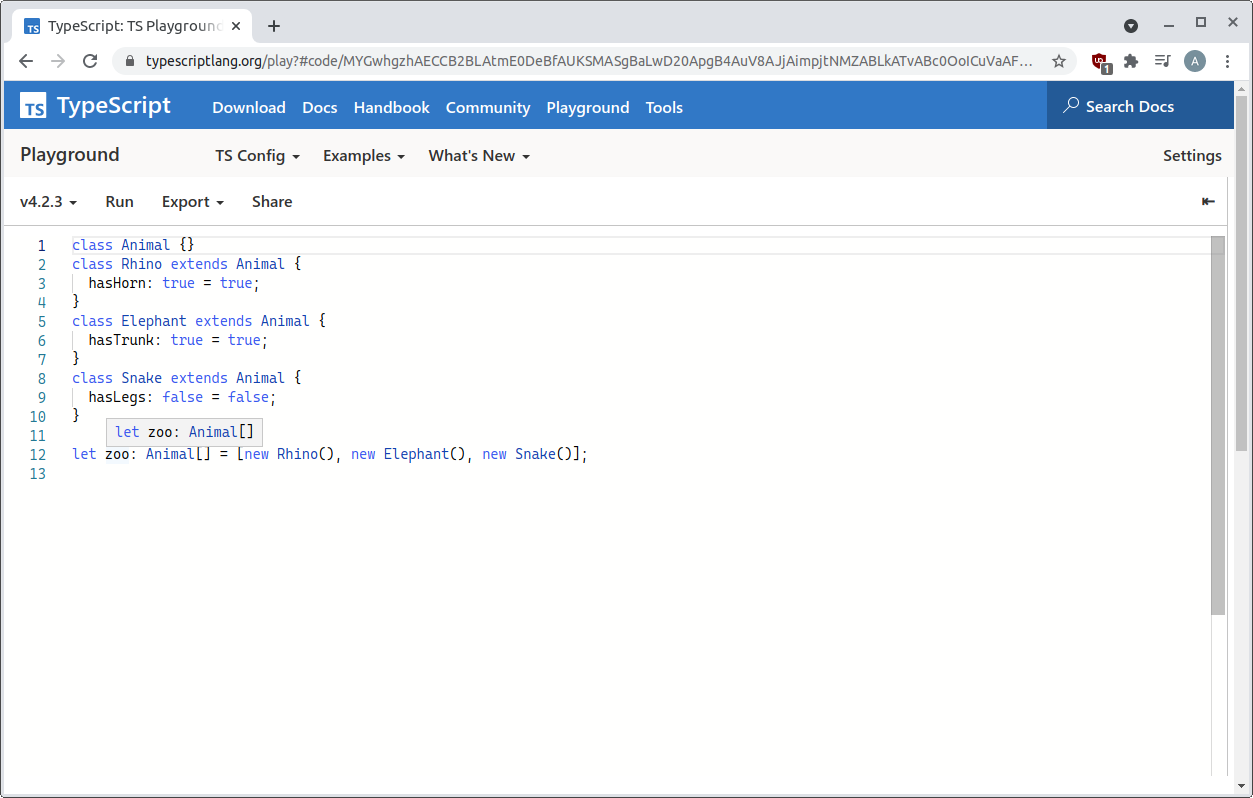
\includegraphics[width=0.467\linewidth]{images/image5.png}
\end{figure}
where C is a set of type functions such as \mintinline{text}{|->|}, \mintinline{text}{|List|} and \mintinline{text}{|Maybe|}.

TODO: latexify the above, replace alpha with tn

For a type to be valid all functions must be fully applied, unlike expressions where the final expression may be a function.  As with expressions, we can again assume a global context that binds the basics variables like \mintinline{text}{|Bool|} and \mintinline{text}{|Int|}. In Hindley’s original paper only \mintinline{text}{|->|} was considered as a type function (i.e. $C = \{ \rightarrow \}$), however here we explore several type functions that have been found useful in practice.

The type function we’ve already been using is \mintinline{text}{|->|} (the \textit{function} type function). It takes two types as arguments and represents a function from the first type to the second. A function from \mintinline{text}{|Int|} to \mintinline{text}{|Bool|} is represented by \mintinline{text}{|(->) Bool Int|} in prefix notation, although would more commonly be written infix as \mintinline{text}{|Bool \rightarrow Int|}.

The function type function (\mintinline{text}{|->|}) should not be confused with the function type: an expression representing a function has a function type, and that function type is the function type function applied to arguments. For example \mintinline{text}{|$\lambda$x. x + 3|} has a function type \mintinline{text}{|Int \rightarrow Int|}, which is the function type function \mintinline{text}{|->|} applied to arguments \mintinline{text}{|Int|} and \mintinline{text}{|Int|}.

The list type function is also very common, which given one type argument represents a list of those types. A list of booleans might be written \mintinline{text}{|List Bool|} or \mintinline{text}{|[] Bool|} in prefix notation, although often the list type is represented by wrapping the type argument in square brackets instead like \mintinline{text}{|[Bool]|}.

\mintinline{text}{|Maybe|} is another type function commonly used in functional languages like Haskell. A \mintinline{text}{|Maybe|} represents the optional presence of something, similar to Java’s \mintinline{text}{|Optional|} and C++’s \mintinline{text}{|std::optional|}. Applied to a boolean type this may be written \mintinline{text}{|Maybe Bool|}, representing a wrapper around nothing or a boolean. In Java this would be represented with a generic as \mintinline{text}{|Optional<Boolean>|} and in C++ as \mintinline{text}{|std::optional<bool>|}.

A similar common type function is \mintinline{text}{|Either|}, which takes two type arguments and represents a wrapper around either one of the types. For example, an either for a boolean or integer is written \mintinline{text}{|Either Bool Int|}.

Finally, tuples represent a defined-length sequence of elements of specific types. Tuple constructors are a set of type functions representing a cross product of their type arguments, named \mintinline{text}{|,|}, \mintinline{text}{|,,|}, \mintinline{text}{|,,,|} and so on for different element lengths. A 3-tuple holding a boolean, integer and integer can technically be written in prefix notation as \mintinline{text}{|(,,) Bool Int Int|} but instead generally tuples borrow mathematical syntax with parentheses and commas like \mintinline{text}{|(Bool, Int, Int)|}.

The set of types made from \mintinline{text}{|var\_t|} and \mintinline{text}{|app\_t|} are known as monotypes. For example, \mintinline{text}{|Bool|}, \mintinline{text}{|Int|}, \mintinline{text}{|Bool \rightarrow Int|}, and \mintinline{text}{|Bool \rightarrow [(Bool, Int \rightarrow Maybe Bool)]|} are all monotypes.

Adding zero or more for-all quantified type variables to monotypes forms polymorphic types or polytypes (called principal type schemes by Hindley). This can be thought of as the \mintinline{text}{|abs|} equivalent for types, written as \mintinline{text}{|\forall a. \rho|} where \mintinline{text}{|\rho|} is a polytype. This definition makes monotypes a special case of polytypes: monotypes are polytypes with zero for-all qualified type variables. We can therefore consider ‘type’ to mean ‘polytype’. By convention, we use $t0, t1, t2, \dots$ for free type variables, and $a, b, c, \dots$ for for-all quantified type variables.

\begin{figure}[h!]
  \centering
  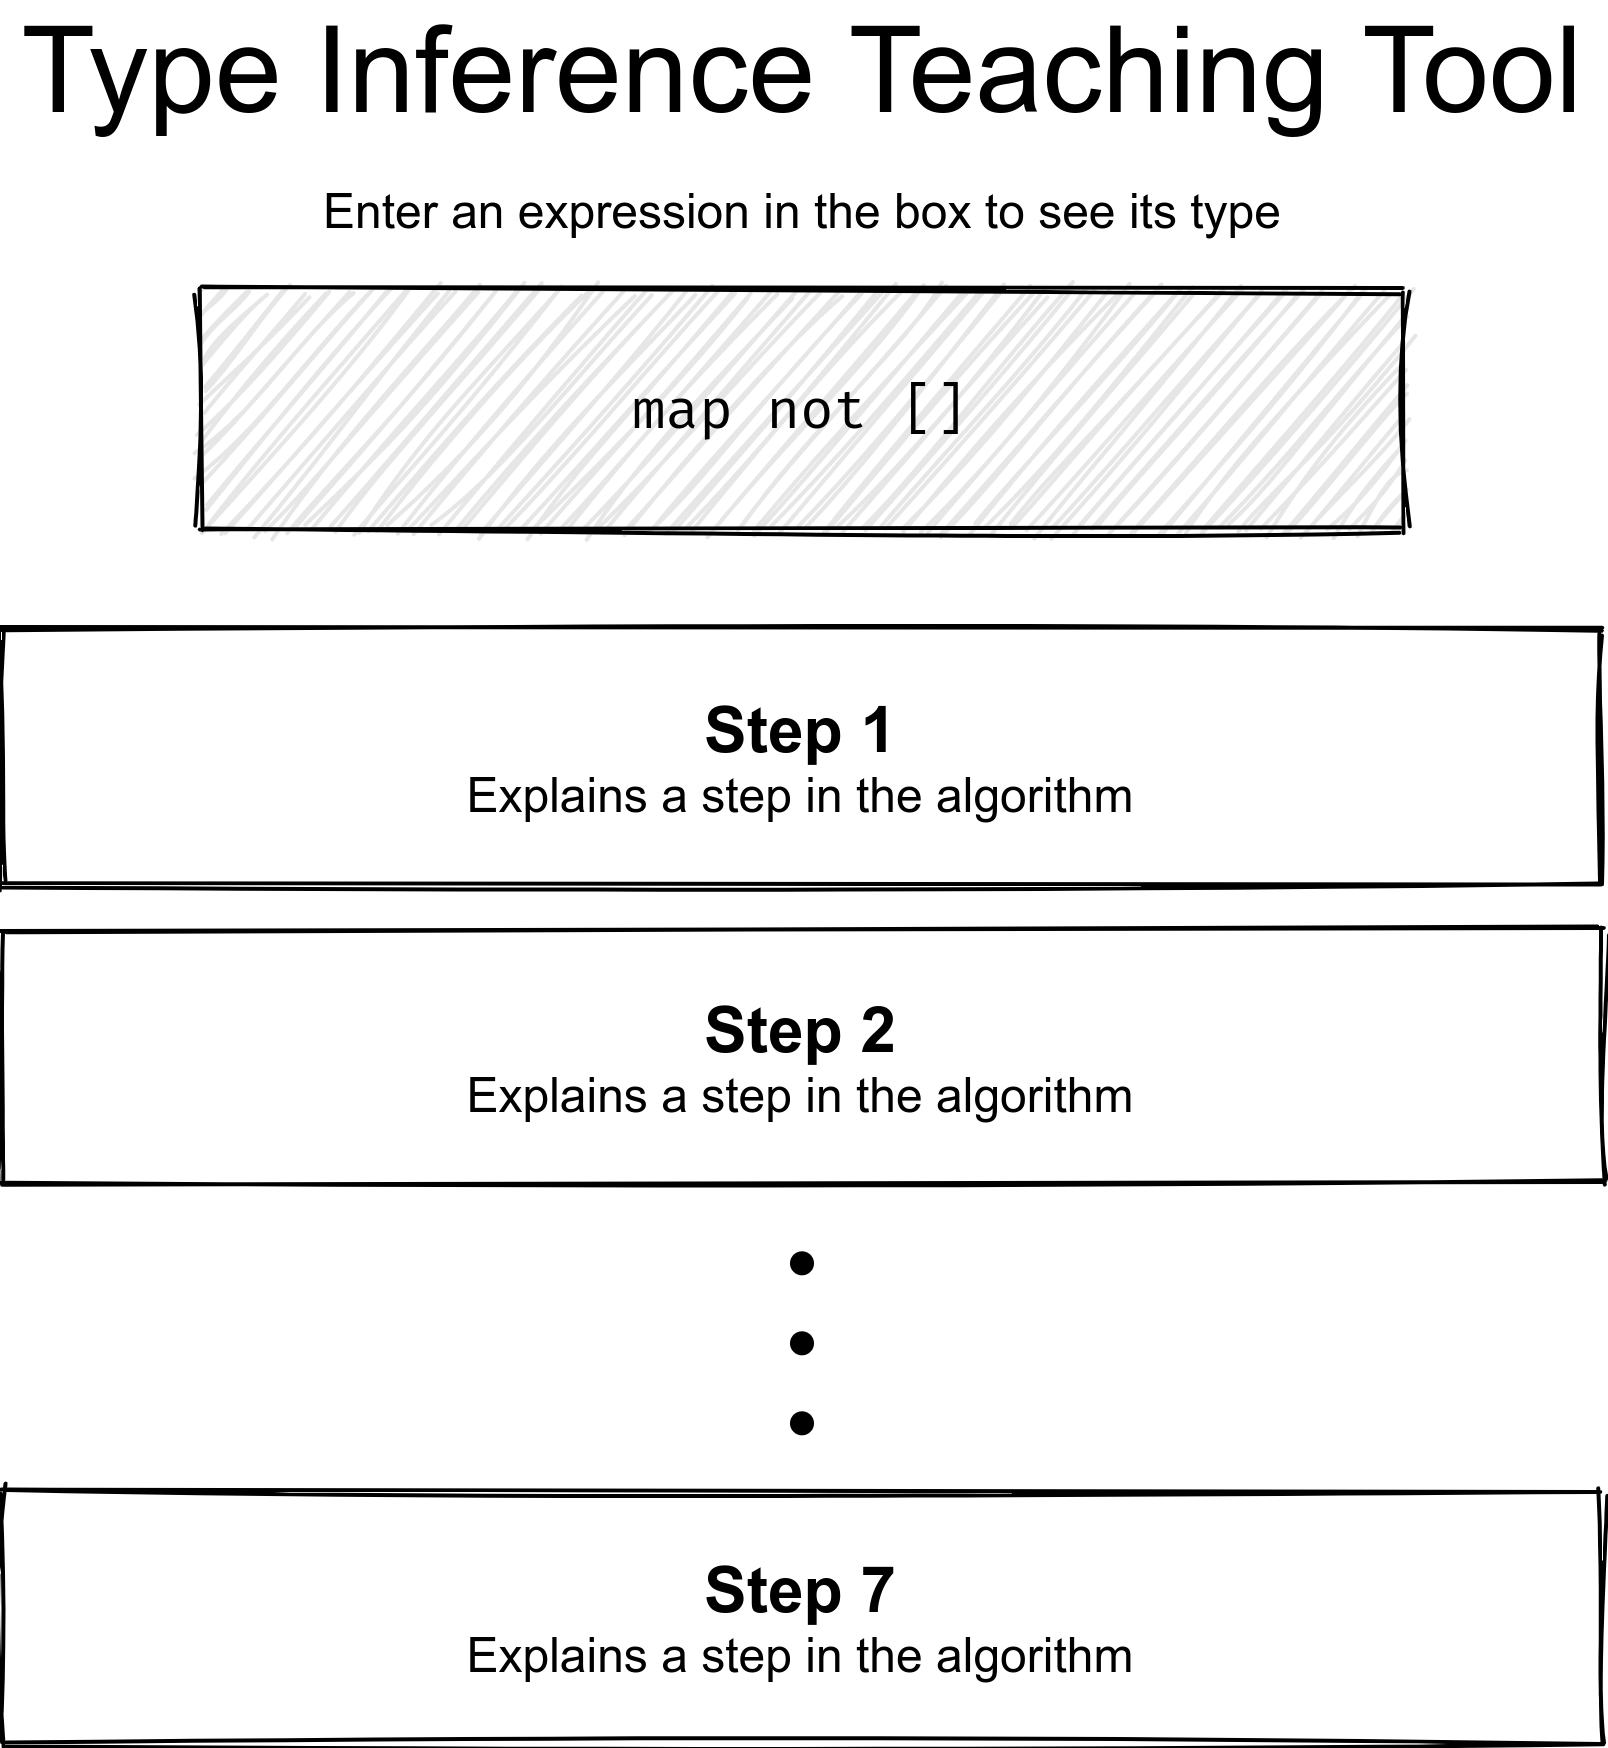
\includegraphics[width=0.290\linewidth]{images/image10.png}
\end{figure}

TODO: latexify the above, but use rho instead of sigma and a instead of alpha

Polytypes allow for parametric polymorphism, where a type may be parameterized by a for-all bound quantifier. This allows functions to accept different types as long as they meet certain constraints. For example the \mintinline{text}{|length|} function is polymorphic: it has the polytype \mintinline{text}{|\forall a. [a] \rightarrow Int|}, which accepts a list of any type and returns its length as an integer. It accepts different types such as \mintinline{text}{|[Bool]|} and \mintinline{text}{|[Int]|} as both of these meet the constraint of being a list.

Correctly inferring polymorphic types can be difficult, and in fact~\cite{ref14} proved that doing so for System F, a type system similar to Hindley-Milner with fewer typing rule constraints, is undecidable. To prevent undecidability, HM avoids overusing polytypes, using only monotypes for \mintinline{text}{|var|}, \mintinline{text}{|con|}, \mintinline{text}{|app|} and \mintinline{text}{|abs|} expressions.

To allow for some polymorphism, \mintinline{text}{|let|} expressions’ parameters are polymorphic in the \mintinline{text}{|let|} body. The process by which the monomorphic parameter type is turned into a polymorphic one is known as generalisation. The overall type of \mintinline{text}{|let|} expressions themselves are not generalised.

This is the difference between:
\begin{itemize}
  \item \mintinline{text}{|let i = (\lambda x \rightarrow x) in (i 3, i True)|} type-checks, as i is generalised to the polytype \mintinline{text}{|\forall a. a \rightarrow a|} within the body \mintinline{text}{|(i 3, i True)|} so can be applied to both an \mintinline{text}{|Int|} and \mintinline{text}{|Bool|}
  \item \mintinline{text}{|(\lambda i \rightarrow (i 3, i True)) (\lambda x. x)|} does not type-check as the function abstraction \mintinline{text}{|(\lambda x. x)|} has the monotype \mintinline{text}{|t0 \rightarrow t0|}, and \mintinline{text}{|t0|} must take only one type in both tuple parts - it cannot be both an \mintinline{text}{|Int|} and a \mintinline{text}{|Bool|}.
\end{itemize}

Hindley-Milner is the basis for the type system of Standard ML \citep{ref15} (which OCaml and F\# are related to) and was the basis of the type system in Haskell \citep{ref16}. It has influenced the development of Rust and Swift, and more generally type inference is present in many more languages including Java, JavaScript and C++.

Haskell has since been extended with type-class constraints \citep{ref17}, functional dependencies \citep{ref18}, and generalised algebraic data types (GADTs) \citep{ref19}. Haskell’s inference engine was moved onto a new engine, OutsideIn(X), when GHC 7.2 was released November 2011 after~\cite{ref20} proposed a solution to the issues with Hindley-Milner’s poor performance on large programs and difficulty inferring expressions without principal types that arise with type-class constraints and GADTs. In doing this, Haskell stopped automatically generalising variables bound by \mintinline{text}{|let|} expressions after~\cite{ref21} argued that generalising \mintinline{text}{|let|} bindings is complex in type inference engines other than HM and the feature was rarely used in practice, with the change only affecting 0.13\% lines of the GHC core libraries. This change does however take it further away from performing HM-like type inference.

Rust’s compiler, rustc, did at one time use a variant of HM for type inference. However,~\cite{ref22} proposed a new scheme which was later implemented to simplify how the compiler reasoned about types. Similarly to Haskell’s move to OutsideIn(X), the new type inference reduces flexibility in some edge cases, although practically this is rare. Both rustc and Rust’s core libraries compiled under the new type inference scheme without changes. Later on,~\cite{ref23} developed chalk, a library designed to be used in rustc to help implement Rust’s generics. This library makes heavy use of unification, a key component of many HM type inference algorithms.

Apple’s Swift heavily uses type inference. It is implemented using a “constraint-based type checker that is reminiscent of the classical Hindley-Milner type inference algorithm” \citep{ref24}. Like other languages it extends HM with additional language features, such as more expressive polymorphic types with additional constraints. To adapt HM to a procedural language, and for improved performance and better error messages, Swift limits type inference to individual statements rather than entire programs.

In addition to their own inference engines, many languages allow the programmer to add more type information through explicit type annotations or casting. This is particularly helpful where the programmer knows more than the type inference algorithm about the limits on how a part of a program will be used.

Java allows casting objects and TypeScript has its \mintinline{text}{|as|} type assertion operator. Programmers can use these sparingly (and often in combination with \mintinline{text}{|instanceof|} and \mintinline{text}{|typeof|} operators respectively) as an escape hatch to work around the type inference algorithm’s limitations. In these situations statements may not be able to be type checked at compile-time so instead runtime checks are performed to maintain type safety.

Java allows casting an object to a subclass \citep{ref25}. Runtime checks are performed, which throw a \mintinline{text}{|ClassCastException|} in case the object is not actually an instance of the subclass.

\begin{minted}[breaklines]{java}
// Dog and Cat extend Animal

Animal c1 = new Dog();
Dog s1 = (Dog) c1; // okay

Animal c2 = new Cat();
Dog s2 = (Dog) c2; // throws ClassCastException at runtime
\end{minted}

TypeScript allows for casting compatible objects with its \mintinline{text}{|as|} operator, or overriding the compile-time type checking completely with a \mintinline{text}{|@ts-ignore|} comment. The following shows that some type-safe code is rejected by the TypeScript type checker, but with several possible workarounds.

\begin{minted}[breaklines]{typescript}
const a = Math.random() < 0.5 ? 'cs310' : 310; // has type "cs310" | 310
const b = a + a; // throws a type error, but b could have type "cs310cs310" | 620

const c = a == 'cs141' ? a + a : a + a; // okay, has type number | string
const d = a as any + a; // okay, has type any
const e = a as any + a as 'cs310cs310' | 620 // okay, has type "cs310cs310" | 620
// @ts-ignore
const f: 'cs310cs310' | 620 = a + a; // okay, has type "cs310cs310" | 620
\end{minted}

TODO: (maybe?) Add section on TypeScript/Elm?

\underline{\href{https://aaltodoc.aalto.fi/bitstream/handle/123456789/42719/master\_Mikkonen\_Juuso\_2020.pdf}{https://aaltodoc.aalto.fi/bitstream/handle/123456789/42719/master\_Mikkonen\_Juuso\_2020.pdf}}
Talks about statically typed languages in JavaScript-land. Mentions things like TypeScript don’t use HM because JS has a lot of structural typing (i.e. if objects have the right properties it’s fine to call methods that depend on that interface) and subtyping.

While real-world languages don’t work exactly like HM, for the purposes of the teaching tool HM gives a good representation of how type inference works to students. HM avoids being too complex to understand, and is still related to how languages commonly used in practice perform type inference.
\subsection{Hindley-Milner type inference}\label{id:h.admfqf7bhkct}
Various algorithms are available to infer types in Hindley-Milner such as Algorithm W by~\cite{ref26} and Algorithm M by~\cite{ref27}. Algorithm W takes a bottom-up approach, attempting to infer the types of subexpressions up the abstract syntax tree, while Algorithm M takes a top-down approach, inferring types down the tree. Algorithm W’ is a minor extension to Algorithm W, by~\cite{ref28} which can improve the quality of type errors raised.

Substitutions are a key concept from logic used by the algorithms. These are maps from variables to terms. When applied to an expression, the variables are substituted with their corresponding terms. In the case of type inference, the variables are type variables, the terms are monotypes and expressions are types.

TODO: fix this latex

Substitutions are represented with curly braces, with each entry separated by a comma and the variables and terms separated with an arrow. For example, $\{ t0 \mapsto t1, t2 \mapsto (Int, Bool) \}$ would replace $t0$ with $t1$, and replace $t2$ with $(Int, Bool)$. Applied to the type $t0 \rightarrow t1 \rightarrow t2$ results in $t1 \rightarrow t1 \rightarrow (Int, Bool)$.

When applying substitutions replacements are performed simultaneously, meaning each variable in the expression may be mapped at most once. For example the substitution $S = \{ t0 \mapsto t1, t1 \mapsto t2 \}$ applied once to the expression $t0$, as $S(t0)$ results in $t1$, not $t2$. Applying the substitution twice, $S(S(t0))$ would result in $t2$.

Any number of substitutions may be applied to expressions. For example, given $S\_1 = \{ t0 \mapsto t2, t1 \mapsto t3 \}$ and $S\_2 = \{ t0 \mapsto t1 \}$, we may apply both to an expression $t0$. Note that this is not commutative, $S\_1(S\_2(t0)) = t3$ while $S\_2(S\_1(t0)) = t2$.

Substitutions may be combined to have the same effect as applying them in order to an expression $E$. For example, with $S\_1 = \{ t0 \mapsto t2, t1 \mapsto t3 \}$ and $S\_2 = \{ t0 \mapsto t1 \}$ again, $combine(S\_1, S\_2)(\rho) = S\_1(S\_2(\rho)) = \{ t0 \mapsto t3, t1 \mapsto t3 \}(\rho)$. As application is not commutative, the order substitutions are combined in matters, i.e. $combine(S\_1, S\_2)$ does not necessarily equal $combine(S\_2, S\_1)$. Combining substitutions is however associative, as $combine(S\_1, combine(S\_2, S\_3))(\rho) = S\_1(S\_2(S\_3(\rho))) = combine(combine(S\_1, S\_2), S\_3)(\rho)$.

A substitution is said to unify two expressions if when applied to both it results in equal expressions. For example, $\{ t0 \mapsto Int, t1 \mapsto Bool \}$ unifies $(t0, Bool)$ and $(Int, t1)$, as when the substitution is applied to either expression the result is $(Int, Bool)$.

Unification is the process of finding unifying substitutions given two expressions, or reporting no such substitution exists.~\cite{ref29} presents a simple algorithm for unification, and~\cite{ref30} and~\cite{ref31} set out linear time unification algorithms.

In the type inference algorithms W, W’ and M, unification is applied to pairs of monotypes. This results in substitutions which effectively combine the various type constraints giving us a final type.

For example, take an expression satisfying two type constraints: it matches the monotype $[Bool] \rightarrow t0$ and it matches with the monotype $[t1] \rightarrow t1$. These constraints might arise in evaluating the type of \mintinline{text}{|head [True]|}. The first constraint is from knowing \mintinline{text}{|[True]|} is a $[Bool]$ so the function should accept a $[Bool]$. The second constraint is based on the known definition of \mintinline{text}{|head|} in the global context. Unification can find the unifying substitution $\{ t0 \mapsto Bool, t1 \mapsto Bool \}$, giving the overall type $[Bool] \rightarrow Bool$. We can then see the resultant type of \mintinline{text}{|head [True]|} is $Bool$.

If at any point unification is not possible, the type constraints must be incompatible and so a type error is raised. For example, there is no unifying substitution for $Int \rightarrow t0$ and $Bool \rightarrow t1$ as one is a function accepting an $Int$ and the other accepts a $Bool$.

For practical purposes, in type inference algorithms we require unifying substitutions to be finite as infinite types are difficult to represent and reason about. For example \mintinline{text}{|x|} in \mintinline{text}{|$\lambda$x. x x|} needs to be a function that accepts itself. Initially assuming \mintinline{text}{|x|} has type $t0 \rightarrow t1$ and knowing it should accept itself, it also has type $(t0 \rightarrow t1) \rightarrow t1$. It also must accept that, so has type $((t0 \rightarrow t1) \rightarrow t1) \rightarrow t1$, $(((t0 \rightarrow t1) \rightarrow t1) \rightarrow t1) \rightarrow t1$, and so on. This is an infinite type and is not allowed by HM. Note that this does not exclude functions from HM which do accept themselves, such as the identity function \mintinline{text}{|id|} with its finite type $\forall a. a \rightarrow a$, as long as they themselves have finite types.

Detecting infinite types in unification is done by checking whether the types are not equal and one of the types occurs in another. This is known as the occurs check. In the previous example \mintinline{text}{|$\lambda$x. x x|} we might try to unify $t0 \rightarrow t1$ with $t0$. $t0$ occurs in $t0 \rightarrow t1$ so there is no finite unifying substitution (an infinite unifying substitution is $\{ t0 \mapsto ((((t0 \rightarrow t1) \rightarrow t1) \rightarrow \text\{infinite \}t1\text\{s\}\dots) \rightarrow t1) \}$). The occurs check failing necessarily means we have an infinite type: the type contains itself.

Inferring types is done in a typing context. Languages often have a global context with built-in functions and their types pre-defined, such as Haskell’s Prelude and JavaScript’s global objects.

Typing contexts can be seen as maps from variable names to their corresponding types, and are represented with the symbol $\Gamma$. For example a context with some common functions may be written $\Gamma = \{ not: Bool \rightarrow Bool, odd: Int \rightarrow Bool, id: \forall a. a \rightarrow a \}$.

Constructs that bind variables like \mintinline{text}{|let|} and \mintinline{text}{|abs|} add entries to a local context for these additional bindings, used in the construct bodies. For example, in \mintinline{text}{|let x = 3 in odd x|} the binding $x: Int$ may be added to the context used to perform type inference on the body subexpression \mintinline{text}{|odd x|}. Similarly in \mintinline{text}{|\x \rightarrow not x|} the binding $x: t0$ may be added to the context for inferring the type of the function body \mintinline{text}{|not x|}. Adding a binding to the context is represented by a $+$, so given $\Gamma = \{ x: Bool \}$ then $\Gamma + y: Int$ is $\{ x: Bool, y: Int \}$.

Applying a substitution to a context is to apply the substitution to every type in the context, or effectively every ‘value’ in the key-value map. For example, applying the substitution $S = \{ t0 \mapsto t1, t2 \mapsto Int \}$ to the context $\Gamma = \{ x: t0, y: t1, z: t2 \}$, results in a new context $S(\Gamma) = \{ x: t1, y: t1, z: Int \}$.

Some types are considered more general than others. A type $\rho\_a$ is more general than a type $\rho\_b$ if there exists a substitution from $\rho\_a$ to $\rho\_b$ whose variables are for-all quantified in $\rho\_a$. This is denoted by $\sqsubseteq$, for example $\forall a. a \rightarrow a$ is more general than $Int \rightarrow Int$ by the substitution $\{ a \mapsto Int \}$, written $\forall a. a \rightarrow a \sqsubseteq Int \rightarrow Int$. Substitutions may (and often do) substitute quantified type variables with free type variables like $t0$ and $t1$, rather than concrete types like $Int$ and $Bool$. As an example, $\forall a \forall b. (a \rightarrow b) \rightarrow [a] \rightarrow [b] \subseteq \forall a. (a \rightarrow Bool) \rightarrow [a] \rightarrow [Bool] \subseteq (t0 \rightarrow Bool) \rightarrow [t0] \rightarrow [Bool]$, following substitutions $\{ b: Bool \}$ and $\{ a: t0 \}$.

For any type $\rho \subseteq \rho$, as the substitution may be empty. A type is strictly less general ($\sqsubset$) than another if and only if the substitution is non-empty. This means a strictly less general type must have at least one fewer quantified variables as one for-all quantified variable must be substituted away.

TODO: (maybe) partial order diagram of some of $\forall a \forall b. (a \rightarrow b) \rightarrow [a] \rightarrow [b]$’s partial and full instantiations.

An expression with a type $\rho\_1$ more general than another type $\rho\_2$ can be considered to have the less general type $\rho\_2$. This means if an expression with type $\rho\_2$ is needed, providing an expression with type $\rho\_1$ will type-check if and only if $\rho\_1 \sqsubseteq \rho\_2$.

The process of giving an expression a less general type is known as instantiation of a type. For example, the type of \mintinline{text}{|id|}, $\forall a. a \rightarrow a$, can be instantiated as all of $Int \rightarrow Int$, $Bool \rightarrow Bool$, $t0 \rightarrow t0$ or even $([t0] \rightarrow (Int, Bool)) \rightarrow ([t0] \rightarrow (Int, Bool))$ and more.

The ‘opposite’ to instantiation is generalisation, where an expression with a certain type can be considered to have a more general type, adding a for-all quantification of a variable. This is allowed where the type variable is not free in any of the types in the context. Not being free in the context means the type variable does not appear unbound anywhere except in the type being generalised itself, so it does not have any other type constraints. Being free of any type constraints, it may be any type and therefore for-all quantified.

Given a type $t0 \rightarrow t1 \rightarrow t2 \rightarrow t3$ and a context $\{ x : t1, y : [t2] \rightarrow Int, z: \forall t3. t3 \}$ we may generalise to $\forall t0 \forall t3. t0 \rightarrow t1 \rightarrow t2 \rightarrow t3$. $t0$ is not in any of the types in the context, and $t3$ is only found bound as a for-all quantified variable. Therefore both of these may be for-all quantified. Both $t1$ and $t2$ are free in the context, so may not be generalised. (Note we’re disregarding our convention of using $a, b, c, \dots$ for for-all quantified variables here, to be strict to the typing rules. Renaming the type variables with $\alpha$-conversions could be done after generalisation to maintain the type variable naming conventions.) Given a context and type, the function $generalise$ returns the fully generalized type possible in that context.

Our five key syntax rules plus instatitation and generalisation give us nine typing rules. Many presentations of Hindley-Milner do not include literal constants in their syntax, or do not explicitly type them given their triviality. Here we give them for completeness.

 \begin{figure}[h!]
  \centering
  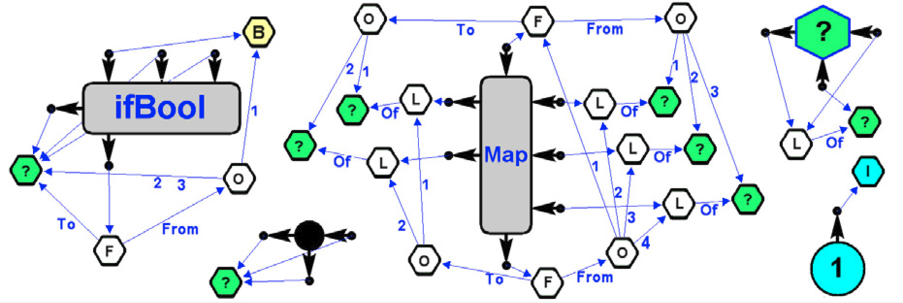
\includegraphics[width=0.505\linewidth]{images/image4.png}
\end{figure}

---------- [Const\_i]
c\_i : Int

-------------- [Const\_c]
c\_c : Char

-------------- [Const\_b]
c\_b : Bool

TODO: latexify the above, replacing sigma with rho

These typing rules can be used to deduce and prove the types of expressions. For example, the expression \mintinline{text}{|not True|} in a context $\Gamma = \{ not: Bool \rightarrow Bool \}$:

$\Gamma \vdash not : Bool \rightarrow Bool [Var]$
$\vdash True : Bool [Const\_b]$
$\Gamma \vdash not True : Bool [App]$

Despite this, the typing rules themselves aren’t an algorithm as they do not specify an order to be applied in. While only one syntax rule can apply to a subexpression, it may be unclear when to apply instantiation and generalisation. Arbitrarily applying rules does not necessarily converge to a solution, as generalisation and instantiation can both continue infinitely. For example repeatedly applying instantiation and generalisation on \mintinline{text}{|id|} with $\Gamma = \{ id: \forall a. a \rightarrow a \}$.

$\Gamma \vdash id : \forall a. a \rightarrow a [Var]$
$\Gamma \vdash id : [t0] \rightarrow [t0] [Inst] (a/[t0])$
$\Gamma \vdash id : \forall b. [b] \rightarrow [b] [Gen]$
$\Gamma \vdash id : [[t1]] \rightarrow [[t1]] [Inst] (b/[t1])$
$\Gamma \vdash id : \forall c. [[c]] \rightarrow [[c]] [Gen]$
$\Gamma \vdash id : [[[t2]]] \rightarrow [[[t2]]] [Inst] (c/[t2])$
$\dots$

The type inference algorithms W, W’ and M effectively are methods to select typing rules to determine a type for the expression, or detect the expression is incorrectly typed. While they don’t apply the typing rules directly, they are close and their respective authors prove they give equivalent results and can be implemented directly.

The algorithms are applied to abstract syntax trees, which represent the expressions in a structured way. For example, an abstract syntax tree for \mintinline{text}{|let y = (\x \rightarrow (odd x)) 3 in not y|} may be visualised as:

TODO: tree diagram of expression

The type inference algorithms are therefore tree traversal algorithms. Generally, they call themselves recursively on subtrees to process subexpressions, and then combine these results to determine a final type (the type of the root node).

Algorithm W is often seen as \textit{the} Hindley-Milner type inference algorithm. Given a context and an expression represented as an abstract syntax tree, W returns a substitution and a monotype.

The purpose of returning the type is obvious, but the purpose of the substitution is less clear. The substitution is a representation of constraints on type variables that have arisen from performing type inference on the expression. For example, given a context $\{ f: t0, not: Bool \rightarrow Bool \}$ and an expression \mintinline{text}{|not (f 3)|} we might return the type $Bool$ and the substitution $\{ t0 \mapsto Int \rightarrow Bool \}$. This substitution is important because if \mintinline{text}{|f|}\mintinline{text}{| |}or the type variable $t0$ are used elsewhere in the same expression we need to type-check those occurrences for consistency with this usage. In a wider expression such as \mintinline{text}{|[not (f 3), f True]|} the substitution from our first subexpression tells us type $t0$ is $Int \rightarrow Bool$. When examining the application of the second \mintinline{text}{|f|}, we find its type from the context which is $t0$, or equivalently now $Int \rightarrow Bool$. We can then raise a type error as we have applied it on a $Bool$.

The algorithm is set out below, for each of the five language constructs. There is a case for each type of node in the abstract syntax tree, so the rule applied at each point is deterministic and easily-chosen based on the node type. Explanations of the more complex cases are given below the algorithm.

\begin{figure}[h!]
  \centering
  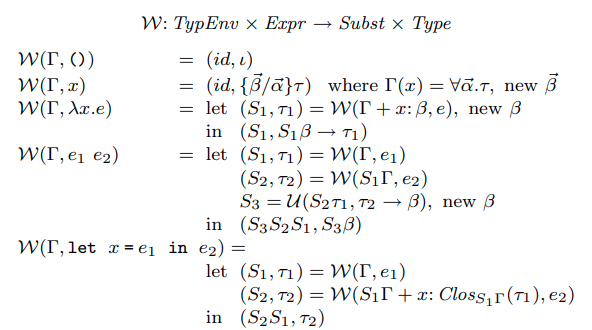
\includegraphics[width=0.987\linewidth]{images/image1.png}
\end{figure}

TODO: latexify the above (taken from Lee), replace () with constants, replace TypeEnv with Context, replace Expr with Expression, replace Subst with Substitution, replace Type with MonoType, replace Clos with generalise, add brackets around applying substitutions, add explicit combines, number the statements, replace id with \{\}, flip ordering of abs and app, replace var rule with let S\_1 = \{ a \mapsto t0, b \mapsto t1, … \}, new t0, t1, … in (id, S\_1\tau) where \Gamma(x) = \forall a \forall b … \tau

The notation $new tn$ specifies that the type variable $tn$ is new (or ‘fresh’), so its name has not been used before. Using globally unique type variables avoids reuse which may incorrectly mix constraints between different types. Most implementations use a global counter, incremented each time a new type variable is needed with names like $t0, t1, t2, \dots$.

The general structure of Algorithm W is to recursively call itself on subexpressions, until the subexpressions are simple leaf nodes. At this point, constant nodes have their assigned type and variable nodes have their type retrieved from the context. The subexpression types are passed back up, where their substitutions are either combined or fed into inferring other subexpressions, and a resultant type is returned.

Case (4app) for function application infers the types of the two subexpressions. It first infers the left one, $e\_1$, then applies the resultant substitution to the context before inferring the right subexpression, $e\_2$. This ensures constraints arising from the $e\_1$ are considered when inferring the second subexpression, so if $e\_1$ and $e\_2$ have conflicting constraints this is detected and a type error is raised. However, this does introduce a left-to-right bias where the type error is raised in the right subexpression if a conflict is found.

Given we know $e\_1$ is a function that should accept $e\_2$’s type, $\tau\_2$, we should be able to unify $\tau\_2 \rightarrow tn$ (a function accepting $\tau\_2$ and returning $tn$ i.e. anything) with the function type $\tau\_1$. We apply the substitution $S\_2$ to $\tau\_1$ when doing this to ensure no constraints have arisen in inferring $e\_2$ that would prevent this unification. Finding a unifying substitution confirms the function application is valid, and we are able to determine the return type (and thus the overall type of this expression) by applying the unifying substitution to the type variable $tn$ used as the return type. If no unifying substitution can be found, the function application is invalid (as the argument type $\tau\_2$ cannot be substituted to reach an accepted type for the function’s type $\tau\_1$) and a type error is raised. Invalid function application (4app) and undefined variables (1var) are the only possible sources of type errors from Algorithm W.

To illustrate, consider \mintinline{text}{|odd 3|} in the context $\Gamma = \{ odd: Int \rightarrow Bool \}$. We find the types of \mintinline{text}{|odd|} and \mintinline{text}{|3|} as $Int \rightarrow Bool$ and $Int$ respectively, unify $Int \rightarrow Bool$ with $Int \rightarrow t0$ to get the substitution $S\_3 = \{ t0 \mapsto Bool \}$ and return the overall type $S\_3(tn) = \{ t0 \mapsto Bool \}t0 = Bool$.

Also consider \mintinline{text}{|odd x|} in the context $\Gamma = \{ odd: Int \rightarrow Bool, x: t0 \}$. Here we find the types of \mintinline{text}{|odd|} and \mintinline{text}{|x|} as $Int \rightarrow Bool$ and $t0$ respectively, unify $Int \rightarrow Bool$ with $t0 \rightarrow t1$ to get the substitution $S\_3 = \{ t0 \mapsto Int, t1 \mapsto Bool \}$ and return the overall type $S\_3(tn) = \{ t0 \mapsto Int, t1 \mapsto Bool \}t1 = Bool$.  In this we also return the substitution $\{ t0: Int, t1: Bool \}$, constraining the external type $t0$ to an $Int$. Given we created $t1$ as a new type variable, it won’t be found elsewhere so does not need to be considered in other expressions so the substitution $\{ t0 \mapsto Int \}$ could equivalently have been returned.

Case (3abs) for function abstraction first infers the type of the function body expression, $e$, by calling W recursively. It passes the current context with an additional binding for the function parameter $x$, assigned to a new type variable with no constraints. This subcall to W for the function body returns the substitution $S\_1$ and type $\tau\_1$. Finally, the substitution $S\_1$ and type $S\_1(tn \rightarrow \tau\_1)$ is returned as the final result for the function abstraction. The type arises from the fact that the function abstraction takes the parameter with the new type $tn$ and returns the type of the body, $\tau\_1$. We apply the substitution $S\_1$ to it to reflect any constraints on the function parameter picked up in the function body.

For an example examine calling W on \mintinline{text}{|\x \rightarrow odd x|} with $\Gamma = \{ odd: Int \rightarrow Bool \}$. The subcall to W calls $W(\Gamma + x: t0, odd x)$ which returns $(S\_1, \tau\_1) = (\{ t0: Int \}, Bool)$. Then $(S\_1, S\_1(tn \rightarrow \tau\_1)) = (\{ t0 \mapsto Int \}, \{ t0 \mapsto Int \}(t0 \rightarrow Bool)) = (\{ t0 \mapsto Int \}, Int \rightarrow Bool)$ is returned as the result.

Case (5let) for let statements first infers the type $\tau\_1$ of the parameter definition, $e\_1$. The parameter type $\tau\_1$ is then generalised with respect to the context to allow for polymorphism as per HM’s type system, before being added to the context as a binding and used to infer the let body $e\_2$. The substitutions $S\_1$ and $S\_2$ are then combined to collect the constraints, and are returned with the let body’s type $\tau\_2$.

Algorithm W’ is a slightly altered variant of Algorithm W, only changing rule (4app) for function application to avoid left-to-right bias.

\begin{figure}[h!]
  \centering
  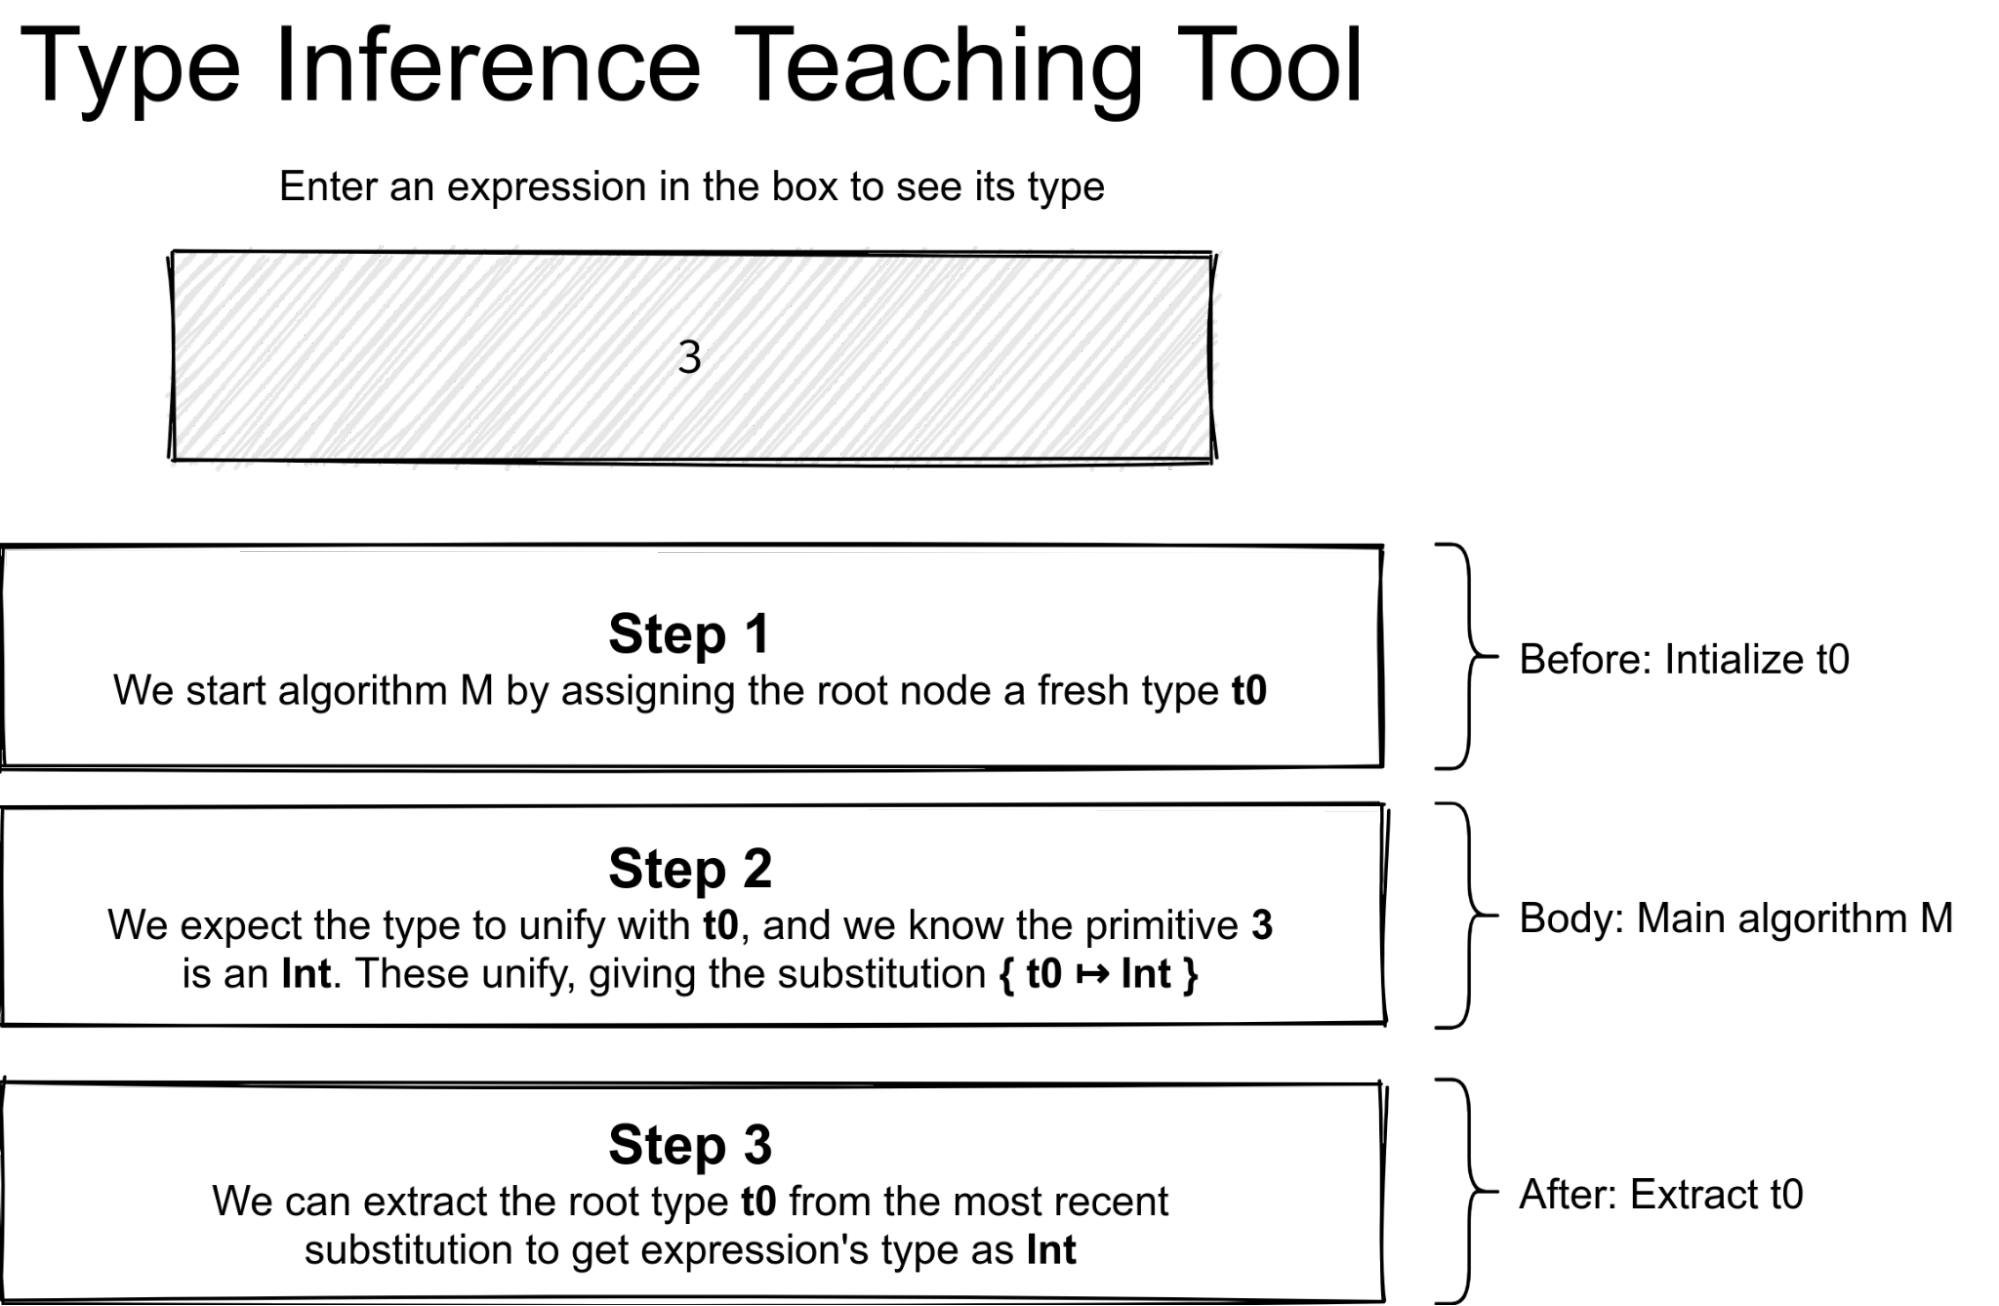
\includegraphics[width=0.782\linewidth]{images/image6.png}
\end{figure}

TODO: write out algorithm in Lee format for W’, 1-index, replace S’ with S\_3, V with S\_4

Algorithm W’ performs substitution unification, introduced in the same paper as W’. Like type unification, substitution unification attempts to find a unifying substitution to unify two values. Unlike type unification, substitution unification attempts to make two substitutions, not types, equal. It returns a unifying substitution, which when combined with either substitution gives the same result, i.e. $combine(unify(S\_1, S\_2), S\_1) = combine(unify(S\_1, S\_2), S\_2)$. Both type and substitution unification is commutative and associative, and may fail if no such substitution exists.

If substitutions share no type variables, finding a unifying substitution can be done by simply combining the substitutions. For example, $unify(\{ t0 \mapsto Int \}, \{ t1 \mapsto Bool \}) = combine(\{ t0 \mapsto Int \}, \{ t1 \mapsto Bool \}) = \{ t0 \mapsto Int, t1 \mapsto Bool \}$.

However, substitution unification generally is different to substitution combination. Combination only simulates the effect of applying consecutive substitutions, so is not concerned with unifying substitution types or maintaining constraints. For example, given $S\_1 = \{ t0 \mapsto t1 \rightarrow Bool \}$ and $S\_2 = \{ t0 \mapsto Int \rightarrow t2 \}$, then $S\_3 = unify(S\_1, S\_2) = \{ t1 \mapsto Int, t2 \mapsto Bool \}$, which is not the same as combining the substitutions. Note the resultant unifying substitution may have a non-empty domain disjoint from both the given substitutions, as in this example. We can see that $combine(S\_3, S\_1) = combine(S\_3, S\_2) = \{ t0 \mapsto Int \rightarrow Bool, t1 \mapsto Int, t2 \mapsto Bool \}$.

Having defined substitution unification, case (4app) in W’ is fairly straightforward. It independently infers the two subexpressions $e\_1$ and $e\_2$, rather than applying $e\_1$’s substitution $S\_1$ to the context before inferring $e\_2$ as in W. The substitutions are then unified and then applied to both subexpression types, ensuring all constraints are applied to both types. The function type and the argument to new type can then be unified in the same way as W.

Algorithm M is a top-down approach to type inference. Implemented as part of an early ML compiler by~\cite{ref32}, it was known as a ‘folklore’ algorithm until~\cite{ref33} formalised it as in the figure below.

Given a context, expression and type it returns a substitution. When compared to W’s signature, this effectively moves the type from the output of W to the input of M. The input type now represents an expected type for the expression, to be checked and then refined by returning a substitution. Types are refined as they progress down the tree (hence top-down), and if they are found to be incompatible at any point a type error is raised. In some cases this can lead to more specific error messages as type errors are generally raised lower down the tree, rather than at potentially more complex function application expressions as in W. More specific error messages are more useful for developers to identify where the bugs are in their programs.

M is initially started at the root node with a new type, i.e. $M(\Gamma, e, tn), new tn$, and the final type can be determined by applying the returned substitution to $tn$. In this way both type inference algorithms can be wrapped to have the signature $Context \times Expression \rightarrow Type$ which would be naturally expected from type inference algorithms.

\begin{figure}[h!]
  \centering
  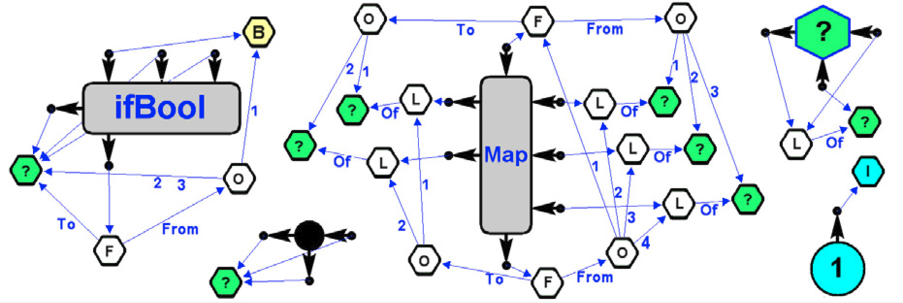
\includegraphics[width=1.000\linewidth]{images/image3.png}
\end{figure}

TODO: latexify the above (taken from Lee), make replacements as per W alg, replace rho with tau\_e

M has some similarities to W, however where W applies unification in function application, M instead pushes this down the tree and performs unification in the leaf nodes and function abstraction.

In rules (1con) and (2var) for constant and variable expressions, we are given an expected type $\tau\_e$ and are verifying it can unify with the literal constant’s type or the type from the context respectively. Unifying in this way returns the type in the substitution, for example $M(\{\}, 3, t0) = unify(Int, t0) = \{ t0: Int \}$ and $M(\{ odd: Int \rightarrow Bool \}, odd, t0 \rightarrow t1) = unify(Int \rightarrow Bool, t0 \rightarrow t1) = \{ t0: Int, t1: Bool \}$, which is passed back up the tree.

Rule (4app) shows function application in M has no unification step. Instead, M is simply called recursively for each expression. The first expression, $e\_1$, is expected to be a function taking a new type variable $tn$ and returning the expected type $\tau\_e$ for the overall application. The second expression should have the argument type for the function, $tn$, after applying substitution $S\_1$ to collect type constraints.

For example, consider \mintinline{text}{|odd 3|} in the context $\Gamma = \{ odd: Int \rightarrow Bool \}$ with expected type $t0$. We call M with the expected type $t1 \rightarrow t0$ on \mintinline{text}{|odd|} to get the substitution $S\_1 = \{ t1: Int, t0: Bool \}$. We then call M with the expected type $S\_1(t1) = Int$ on \mintinline{text}{|3|}, which is validated and returns an empty substitution $S\_2 = \{\}$. Finally, we return the combined substitution $\{ t1: Int, t0: Bool \}$.

In rule (3abs) for function abstraction, we verify the expected type unifies with a new function type. This gives a substitution mapping the variables $t1$ and $t2$ to the expected function types, if any. This is applied to the context, along with adding the parameter $x$’s type as $t1$. We then use M to infer the type of the function body, expecting it to have the unified return type $t2$. We return the combined substitution from both parts.

For an example we look at applying M on \mintinline{text}{|\x \rightarrow odd x|} with $\Gamma = \{ odd: Int \rightarrow Bool \}$ and expected type $t0$. We first unify $t0$ with the new type $t1 \rightarrow t2$, resulting in $S\_1 = \{ t0: t1 \rightarrow t2 \}$. We then make the recursive call to M with the function body \mintinline{text}{|odd x|}, context $\{ odd: Int \rightarrow Bool, x: t1 \}$ and expected type $t2$. This results in the substitution $S\_2 = \{ t1: Int, t2: Bool \}$, which we combine with $S\_1$ to get $combine(S\_2, S\_1) = \{ t0: Int \rightarrow Bool, t1: Int, t2: Bool \}$. As in W’s function application, the new type variables will be unused outside of this expression so we can equivalently exclude $t1$ and $t2$ from the substitution.

Finally, let expressions infer the type of their parameter $e\_1$ with a new type, then infer the type of their body $e\_2$ expecting it to have the overall expected type $\tau\_e$. Similarly to function abstraction, the substitution from the parameter is passed when inferring the body, and combined with the body’s substitution to give an overall result.

These type inference algorithms do have limitations. They all sometimes produce poor type error messages; Algorithm W often detects errors late, highlighting too large of a subexpression to be useful and Algorithm M often detects too specific of a term without context as to what original definition it violates. Algorithm W has the left-to-right bias which Algorithm W’ attempts to correct for, however this can sometimes exacerbate the problem with highlighting large subexpressions. Poor error messages make it difficult for the programmer to understand how to fix the problem.

To improve error messaging, hybrid or constraint-based algorithms along with heuristics are often used in practice to provide more informative error messages. Reducing the size of the amount inferred at once can help make errors more precise. For example, Apple’s Swift uses a bi-directional type inference algorithm on single statements \citep{ref34}.

Additionally, despite not being required in all languages, explicit type annotations are often used to help identify errors earlier at locations which are easier to interpret \citep{ref35}. This is especially common for function definitions or program entry points. This also effectively splits up the program into smaller parts which can be inferred against separately, improving performance and making type errors more precise. In some cases, type inference algorithms struggle with (directly or indirectly) recursively defined functions and type annotations can help define these types. Finally, changing a rigidly-typed interface also highlights potential breaking changes to libraries or helper functions. In this way type annotations act as documentation to future programmers using the code. Manually specified, more specific types may be an improvement over automatically inferred types as sometimes the most general type as worked out by a type inference algorithm may not clearly convey the intent of the programmer.

TODO: (maybe?) Add a section on type errors. Resources:

\underline{\href{https://www.researchgate.net/profile/Jurriaan\_Hage/publication/221241370\_Scripting\_the\_Type\_Inference\_Process/links/02e7e51a37f9233c65000000.pdf}{https://www.researchgate.net/profile/Jurriaan\_Hage/publication/221241370\_Scripting\_the\_Type\_Inference\_Process/links/02e7e51a37f9233c65000000.pdf}}
Improving type error messages

\underline{\href{https://dspace.library.uu.nl/bitstream/handle/1874/7297/full.pdf?sequence=8}{https://dspace.library.uu.nl/bitstream/handle/1874/7297/full.pdf?sequence=8}}
Top quality type error messages

\underline{\href{https://manu.sridharan.net/files/mycroft-preprint.pdf}{https://manu.sridharan.net/files/mycroft-preprint.pdf}}
A Practical Framework for Type Inference Error Explanation

\underline{\href{http://citeseerx.ist.psu.edu/viewdoc/download?doi=10.1.1.110.5050\&rep=rep1\&type=pdf}{http://citeseerx.ist.psu.edu/viewdoc/download?doi=10.1.1.110.5050\&rep=rep1\&type=pdf}}
PhD thesis which talks about hindley milner and type inference errors a lot
\section{Design}\label{id:h.7ggvdxb04tzm}
- different ui mockups
- different structures
- different libraries

\underline{\href{https://www.sigmacomputing.com/blog/writing-a-parser-combinator-from-scratch-in-typescript/}{https://www.sigmacomputing.com/blog/writing-a-parser-combinator-from-scratch-in-typescript/}}
Parser in TypeScript

\underline{\href{https://tomassetti.me/parsing-in-javascript/}{https://tomassetti.me/parsing-in-javascript/}}
Parsing in JavaScript - lots of library recommendations (see Parjs and Jison)
\section{Implementation}\label{id:h.igepudpadp49}
Developed gdoc2latex

Set up CI system to build latex docs

Tried using Docker to run latex compilation step in GitHub actions, but found it was significantly slower (2 mins vs 45 seconds) than installing texlive-latex-extra and texlive-bibtex-extra on the runner directly.

Implemented algorithm W in a mix of class-based and functions, then reimplemented to be just functions.

Added custom test matcher

How the step logging works

How does the web app work, performance analysis and considerations

Analytics

Adding algorithm M and W’
\section{Evaluation}\label{id:h.e6letww4nhn0}
Maybe also analyse performance?

Compare to existing available libraries?

\subsection{User testing}\label{id:h.bsy9mpun8nk3}
Lay out the aims of user testing, i.e.: (goals increasing in ‘scope’)
- software is accessible and usable
- the results can be understood
- it improves students’ understanding of types and type inference

How the survey was constructed and how that relates to aims

How the survey was distributed and incentivised

How analytics data was collected and how that relates to aims

How participants privacy was protected
\subsubsection{Survey}\label{id:h.yqiowsgjmohq}
Questions:
- Try entering: map odd []. Try to understand the steps. What is the unifying substitution performed in step 3?
- Try entering: not 3. Try to understand the steps. What is the problem found?

TODO: Expand on what options were available for these questions and why

These questions were to verify users were able to access, use and interpret the results of the tool. This helps test the hypothesis that the software was accessible and usable, and that results could be understood.

The first had 91\% of respondents select the correct answer. 2 respondents chose the type distractor, and 1 respondent entered a different substitution. 1 respondent did not understand the output enough.

The second had 100\% of respondents select the correct answer.

In both questions, no respondents selected that they could not access or use the software, and the high correct response rate for both questions support hypotheses 1 and 2.

Questions:
- What is really helpful about this tool?
- What could be improved in this tool?

These questions were to better understand qualitatively what helped students understand type inference, so the tool could be improved. Determining what is most helpful about the tool allows focusing on those parts, while asking what could be improved highlights areas to be changed.

Positive themes found were:
- 2x Function application was explained well, which also helped explain curried functions
- 23x Steps are clear / easy-to-understand
- 15x Steps are well-presented / well-visualised
- 8x Tool explains why invalid expressions are invalid
- 8x Showing substitutions helped explain unification
- Learnt how let syntax worked
- 9x Liked visual design / colour scheme
- Tool helpful for more complex examples
- Liked being able to try different things, felt it was more effective than slides/books
- Examples were helpful
- 13x helped me understand unification
- 11x helped me understand type inference
- 4x helped me understand Haskell
- Application is very fast

Improvement themes found were:
- 2x Information on homepage could be made more obvious
- Contact details on the website could help report bugs, give feedback
- Automatically suggesting typo corrections e.g. ‘Fals’ to ‘False’
- On mobile changing the input expression should not cause the screen to move
- Adding functor and applicative support
- Adding support for list comprehensions
- 5x Adding more general information on the HM type system and the HM algorithm
- 4x Using arrows to navigate through steps rather than scrolling
- 3x Function application step could be made clearer
- 2x Fix typo ‘instatiate’ to ‘instantiate’
- Support infix expressions
- Adding a quiz mode
- 3x Improve wording of function application step
- 2x Adding support for declaring custom types
- Swapping order of AST and explaining content
- 2x Making it clearer the expression box was a text input
- Want input expression to be visible when scrolled down the page
- 1x Disliked colour scheme
- Use more mathematical notation
- 2x Add animation
- Add dark theme
\subsubsection{Analytics}\label{id:h.67g05flyfv0z}

\section{Conclusions and Further Work}\label{id:h.fc67ipatea73}

\section{Ethics}\label{id:h.i0n8c6hqdr6j}

\section{Acknowledgements}\label{id:h.xqaef57orpsv}
This document was typeset using a derivative of the CS310 starter pack\footnote{\href{https://github.com/mbg/cs310}{https://github.com/mbg/cs310}} by Michael Gale, licensed under CC BY 4.0.






































\bibliography{index}

\bibliographystyle{./plainnat}

\end{document}